\section{Transition Rule Dependencies}
\label{sec:sts-rules-overview}

Figure~\ref{fig:sts-rules-dependencies} shows all STS rules, the sub-rules they
use and possible dependencies. Each node in the graph represents one rule, the
top rule being CHAIN.\@ A straight arrow from one node to another one represents
a sub-rule relationship. There are two recursive rules, LEDGERS and DELEGS which
have self loops.

An arrow with a dotted line from one node to another represents a dependency in
the sense that the output of the target rule is an input to the source one,
either as part of the source state, the environment or the signal. In most cases
these dependencies are between sub-rules of a rule. In the case of recursive
rules, the sub-rule can also have a dependency on the super-rule. Those
recursively call themselves while traversing the input signal sequence until
reaching the base case with an empty input sequence.

\begin{figure}[htp]
  \centering
  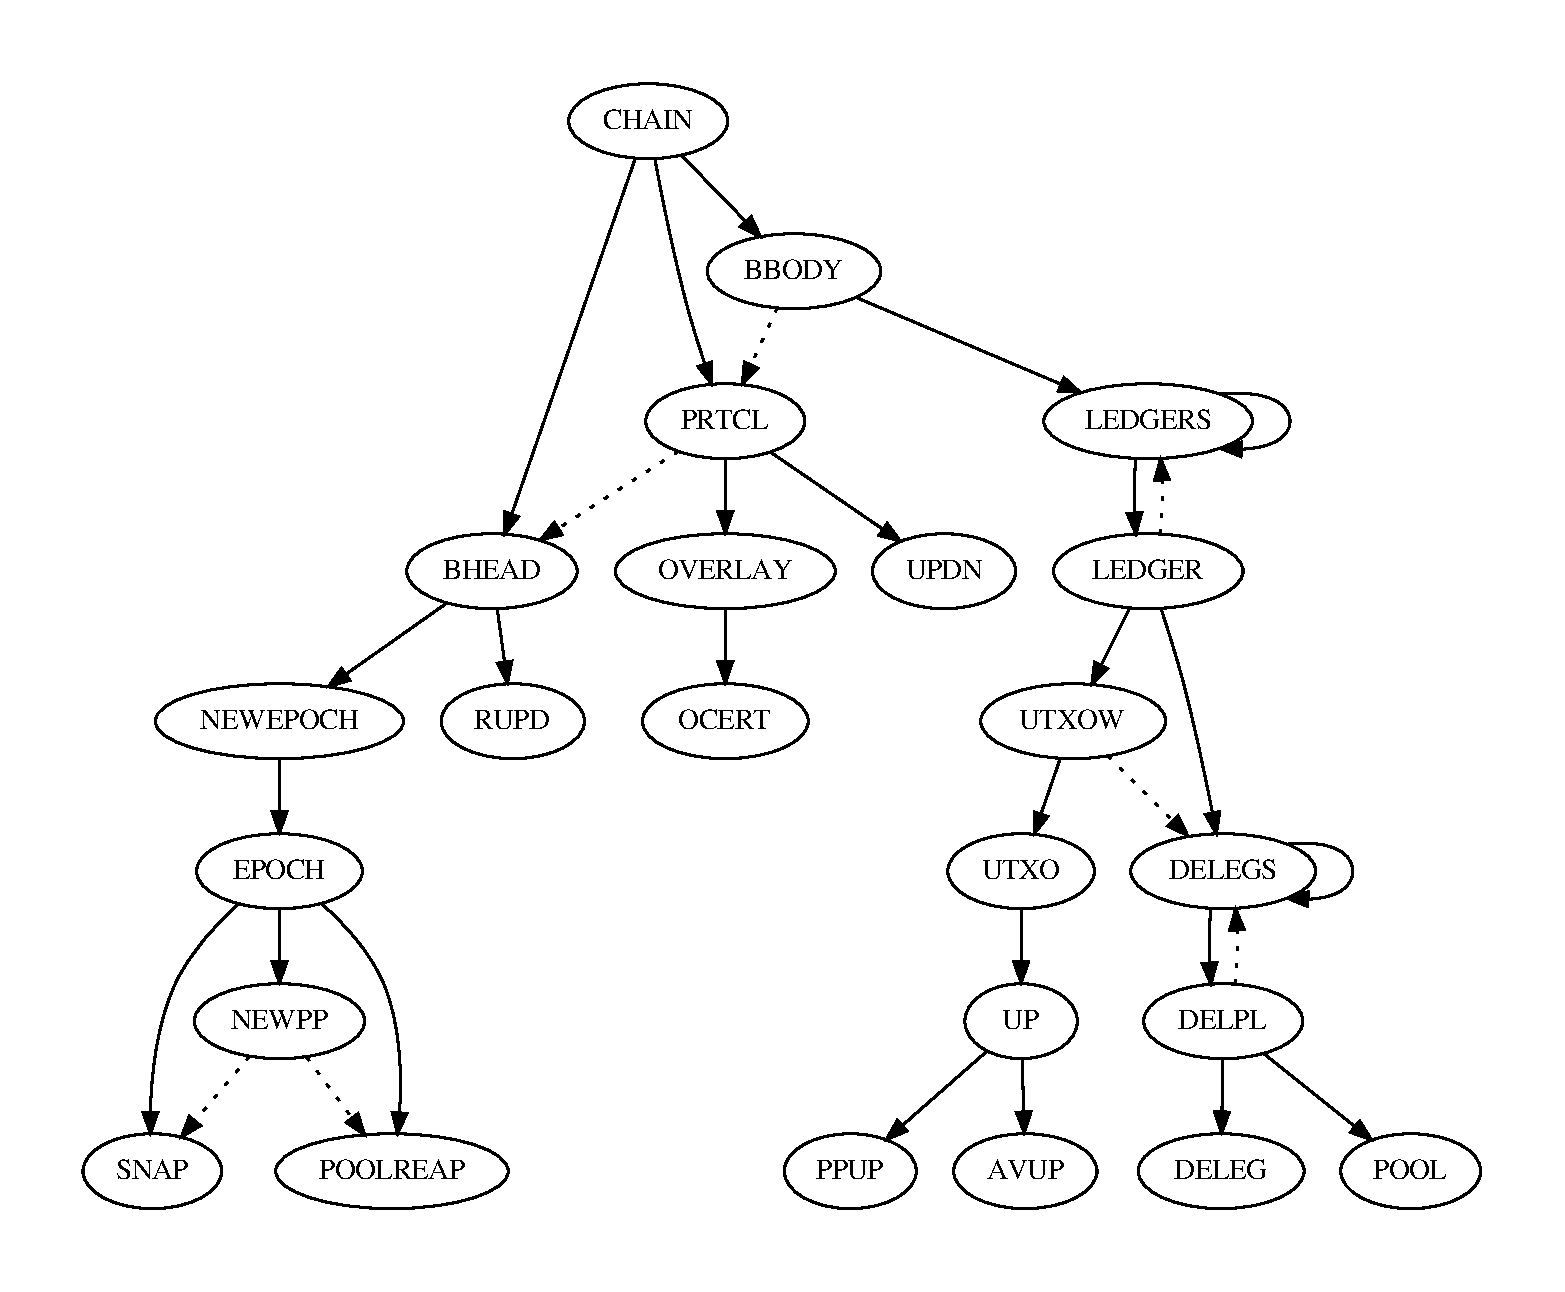
\includegraphics[width=\textwidth]{rules}
  \caption{STS Rules, Sub-Rules and Dependencies}
  \label{fig:sts-rules-dependencies}
\end{figure}

%%% Local Variables:
%%% mode: latex
%%% TeX-master: "ledger-spec"
%%% End:
